\chapter{Results}\label{Results}

%Denote by $\mathbf{x}^J$ the subvector formed from the entries of $\mathbf{x}$ indexed by $J$. 
%A set of $k$-sparse vectors is said to be in \emph{general linear position} when any $k$ of them are linearly independent. 

\section{Definitions}

To state precisely the results of this work, we will require first the identification of some combinatorial criteria on the supports\footnote{Recall that a vector $\mathbf{x}$ is said to be \emph{supported} in $S$ when $\mathbf{x} \in \text{\rmfamily span}\{\mathbf{e}_j: j\in S\}$, with $\mathbf{e}_j$ forming the standard column basis.} of sparse vectors. Let $\{1, \ldots, m\}$ be denoted $[m]$, its power set $2^{[m]}$, and ${[m] \choose k}$ the set of subsets of $[m]$ of size $k$.  A \emph{hypergraph} on vertices $[m]$  is simply any subset $\mathcal{H} \subseteq 2^{[m]}$. Let us say that $\mathcal{H}$ is \textit{$k$-uniform} when $\mathcal{H} \subseteq {[m] \choose k}$. The \emph{degree} $\deg_\mathcal{H}(i)$ of a node $i \in [m]$ is the number of sets in $\mathcal{H}$ that contain $i$, and we say $\mathcal{H}$ is \emph{regular} when for some $r$ we have $\deg_\mathcal{H}(i) = r$ for all $i$ (given such an $r$, we say $\mathcal{H}$ is \textit{$r$-regular}). Let us also write $2\mathcal{H} := \{ S \cup S': S, S' \in \mathcal{H}\}$.  The following class of structured hypergraphs is a key ingredient in this work.

\begin{definition}\label{sip}
Given $\mathcal{H} \subseteq 2^{[m]}$, the \textbf{star} $\sigma(i)$ is the collection of sets in $\mathcal{H}$ containing $i$. We say $\mathcal{H}$ has the \textbf{singleton intersection property} (\textbf{SIP}) when $\cap \sigma(i) = \{i\}$ for all $i \in [m]$. 
\end{definition}

Next, we will require a quantitative generalization of the spark condition (\ref{SparkCondition}) to combinatorial subsets of supports. The \emph{lower bound} of an $n \times m$ matrix $\mathbf{M}$ is the largest $\alpha$ with \mbox{$\|\mathbf{M}\mathbf{x}\|_2 \geq \alpha\|\mathbf{x}\|_2$} for all $\mathbf{x} \in \mathbb{R}^m$ \cite{Grcar10}. By compactness of the unit sphere, every injective linear map has a positive lower bound; hence, if $\mathbf{M}$ satisfies \eqref{SparkCondition}, then submatrices formed from $2k$ of its columns or less have strictly positive lower bounds. 

The lower bound of a matrix is generalized below in (\ref{Ldef}) by restricting it to the spans of certain submatrices\footnote{See \cite{vidal2005generalized} for an overview of the related ``union of subspaces" model.} associated with a hypergraph $\mathcal{H} \subseteq {[m] \choose k}$ of column indices. Let $\mathbf{M}_S$ denote the submatrix formed by the columns of a matrix $\mathbf{M}$ indexed by $S \subseteq [m]$ (setting $\mathbf{M}_\emptyset := \mathbf{0}$).  In the sections that follow, let $\bm{\mathcal{M}}_S$ denote the column-span of a submatrix $\mathbf{M}_S$, and $\bm{\mathcal{M}}_\mathcal{G}$ to denote $\{\bm{\mathcal{M}}_S\}_{S \in \mathcal{G}}$. Define: % Define $L_\mathcal{H}(\mathbf{M})$ as follows:
%\begin{align*} 
%L_\mathcal{H}(\mathbf{M}) := \min \left\{ \frac{ \|\mathbf{M}(\mathbf{x}_1-\mathbf{x}_2)\|_2 }{ \sqrt{2k} \|\mathbf{x}_1-\mathbf{x}_2\|_2} : \mathbf{x}_1, \mathbf{x}_2 \in \cup_{S \in \mathcal{H}} \bm{\mathcal{M}}_S \right\},
%\end{align*} 
%
%where we write $L_{2k}$ in place of $L_\mathcal{H}$ when $\mathcal{H} = {[m] \choose k}$. Note that if $\mathcal{H}$ covers $[m]$, then $L_2 > L_\mathcal{H}$.\footnote{The reader should beware that $L_2 = L_{[m]}$, whereas $L = L_{\{[m]\}}$. For even $k$, the quantity $1 - \sqrt{k} L_k(\mathbf{M})$ is also known in the compressed sensing literature as the (asymmetric) lower restricted isometry constant \cite{Blanchard2011}.} Clearly, for any $\mathbf{M}$ satisfying \eqref{SparkCondition}, we have $L_{k'}(\mathbf{M}) > 0$ for  $k' \leq 2k$.
%\begin{align*}
%L_\mathcal{H}(\mathbf{M}) := \min \left\{ \frac{ \|\mathbf{M}_S\mathbf{x}\|_2 }{ \sqrt{k} \|\mathbf{x}\|_2} : S \in \mathcal{H} \right\},
%\end{align*} 
%\begin{align*}
%L_\mathcal{H}(\mathbf{M}) := \max \left\{ \ falpha: \|\mathbf{M}_S\mathbf{x}\|_2 \geq \alpha \sqrt{k} \|\mathbf{x}\|_2 : S \in \mathcal{H}, \ \ \mathbf{x} \in \mathbb{R}^m \right\},
%\end{align*} 
\begin{align}\label{Ldef}
L_\mathcal{H}(\mathbf{M}) := \min \left\{ \frac{\|\mathbf{M}_S\mathbf{x}\|_2}{ \sqrt{k} \|\mathbf{x}\|_2} : S \in \mathcal{H}, \ \mathbf{0} \neq \mathbf{x} \in \mathbb{R}^{|S|} \right\},
\end{align} 
%
writing also $L_{k}$ in place of $L_\mathcal{H}$ when $\mathcal{H} = {[m] \choose k}$.\footnote{In compressed sensing literature, \mbox{$1 - \sqrt{k} L_k(\mathbf{M})$}  is the asymmetric lower restricted isometry constant for $\mathbf{M}$ with unit $\ell_2$-norm columns \cite{Blanchard2011}.\label{ripfootnote}}  As explained above, compactness implies that $L_{2k}(\mathbf{M}) > 0$ for all $\mathbf{M}$ satisfying \eqref{SparkCondition}. Clearly, $L_{\mathcal{H}'}(\mathbf{M}) \geq L_\mathcal{H}(\mathbf{M})$ whenever $\mathcal{H}' \subseteq \mathcal{H}$, and similarly any $k$-uniform $\mathcal{H}$ satisfying $\cup \mathcal{H} = [m]$ has $L_2 \geq L_{2\mathcal{H}} \geq L_{2k}$ (letting $L_{2k}$ := $L_m$ whenever $2k > m$).

\section{Uniqueness theorems}

\subsection{Deterministic guarantees}

The following is the statement of the main result. For expository purposes the quantity $C_1$ (a function of $\mathbf{A}$, $\mathbf{x}_1, \ldots, \mathbf{x}_N$, and $\mathcal{H}$) will be left undefined until Chap.~\ref{DUT}.

%eps-tightness COUNTER-EXAMPLE:
%Consider the alternate dictionary $B = \left(\mathbf{0}, \frac{1}{2}(\mathbf{e}_1 + \mathbf{e}_2), \mathbf{e}_3, \ldots, \mathbf{e}_{m} \right)$ and sparse codes $\mathbf{b}_i = \mathbf{e}_2$ for $i = 1, 2$ and $\mathbf{b}_i = \mathbf{e}_i$ for $i = 3, \ldots, m$. Then $|A\mathbf{a}_i - B\mathbf{b}_i| = 1/\sqrt{2}$ for $i = 1, 2$ (and $0$ otherwise). If there were permutation and invertible diagonal matrices $P \in \mathbb{R}^{m \times m}$ and $D \in \mathbb{R}^{m \times m}$ such that $|(A-BPD)\mathbf{e}_i| \leq C\varepsilon$ for all $i \in [m]$, then we would reach the contradiction $1 = |P^{-1}\mathbf{e}_1|_2 = |(A-BPD)P^{-1}\mathbf{e}_1|_2 \leq 1/\sqrt{2}$. 

\begin{theorem}\label{DeterministicUniquenessTheorem}
%Fix integers $n, k, m$ and $\overline m$. 
If an $n \times m$ matrix $\mathbf{A}$ satisfies $L_{2\mathcal{H}}(\mathbf{A}) > 0$ for some $r$-regular $\mathcal{H} \subseteq {[m] \choose k}$ with the SIP, and $k$-sparse \mbox{$\mathbf{x}_1, \ldots, \mathbf{x}_N \in \mathbb{R}^m$} include more than $(k-1){\overline m \choose k}$ vectors in general linear position\footnote{Recall that a set of vectors sharing support $S$ are in \emph{general linear position} when any $|S|$ of them are linearly independent.} supported in each $S \in \mathcal{H}$, then the following recovery guarantees hold for $C_1 > 0$ given by \eqref{Cdef1}.

\textbf{Dictionary Recovery:} Fix $\varepsilon < L_{2}(\mathbf{A}) / C_1$.\footnote{Note that the condition $\varepsilon < L_2(\mathbf{A}) /C_1$ is necessary; otherwise, with \mbox{$\mathbf{A}$ = $\mathbf{I}$} (the identity matrix) and $\mathbf{x}_i = \mathbf{e}_i$, the matrix $\mathbf{B} = \left[\mathbf{0}, \frac{1}{2}(\mathbf{e}_1 + \mathbf{e}_2), \mathbf{e}_3, \ldots, \mathbf{e}_{m} \right]$ and sparse codes $\mathbf{\overline x}_i = \mathbf{e}_2$ for $i = 1, 2$ and $\mathbf{\overline x}_i = \mathbf{e}_i$ for $i \geq 3$ satisfy $\|\mathbf{A}\mathbf{x}_i - \mathbf{B}\mathbf{\overline x}_i \|_2 \leq \varepsilon$ but nonetheless violate \eqref{Cstable}.} If an $n \times \overline m$ matrix $\mathbf{B}$ has, for every $i \in [N]$, an associated $k$-sparse $\mathbf{\overline x}_i$ satisfying \mbox{$\|\mathbf{A}\mathbf{x}_i - \mathbf{B}\mathbf{\overline x}_i\|_2 \leq \varepsilon$}, then $\overline m \geq m$, and provided that $\overline m (r-1) < mr$, there is a permutation matrix $\mathbf{P}$ and an invertible diagonal matrix $\mathbf{D}$ such that:
\begin{align}\label{Cstable}
\|\mathbf{A}_j- (\mathbf{BPD})_j\|_2 \leq C_1 \varepsilon, \ \ \text{for all } j \in J,
\end{align}
%
for some $J \subseteq [m]$ of size \mbox{$m - (r-1)(\overline m - m)$}. 
% $\overline m - r(\overline m - m)$

\textbf{Code Recovery:} If, moreover, $\mathbf{A}_J$ satisfies \eqref{SparkCondition} and $\varepsilon < L_{2k}(\mathbf{A}_J) / C_1$, then $(\mathbf{BP})_J$ also satisfies \eqref{SparkCondition} with $L_{2k}(\mathbf{BP}_J) \geq (L_{2k}(\mathbf{A}_J) - C_1 \varepsilon) / \|\mathbf{D}_J\|_1$, and for all $i \in [N]$:
\begin{align}\label{b-PDa}
%\|\mathbf{x}^J_i - \mathbf{D}^{-1}\mathbf{P}^{\top}\mathbf{\overline x}^{\overline J}_i\|_1 &\leq  \left( \frac{ 1+C_1 \|\mathbf{x}^{J}_i\|_1 }{ L_{2k}(\mathbf{A}) -  C_1\varepsilon } \right) \varepsilon \ \  \text{for $i \in [N]$}.
\|(\mathbf{x}_i)_J - (\mathbf{D}^{-1}\mathbf{P}^{\top} \mathbf{\overline x}_i)_J\|_1 &\leq  \left( \frac{ 1+C_1 \|(\mathbf{x}_i)_J\|_1 }{ L_{2k}(\mathbf{A}_J) -  C_1\varepsilon } \right) \varepsilon,
\end{align}
%
where subscript $(\cdot)_J$ here represents the subvector formed from restricting to coordinates indexed by $J$.
\end{theorem}

%We delay defining the explicit constant $C_1$ until Section \ref{DUT} (\eqref{Cdef1}).
%To be clear, the implication of Thm.~\ref{DeterministicUniquenessTheorem} is that $Y = \{\mathbf{Ax}_1, \ldots, \mathbf{Ax}_N\}$ has a stable $k$-sparse representation in $\mathbb{R}^m$, with \eqref{def1} guaranteed provided $\varepsilon$ in Def.~\ref{maindef} does not exceed: 
In words, Thm.~\ref{DeterministicUniquenessTheorem} says that the smaller the regularity $r$ of the original support hypergraph $\mathcal{H}$ or the difference $\overline m - m$ between the assumed and actual number of elements in the latent dictionary, the more columns and coefficients of the original dictionary $\mathbf{A}$ and sparse codes $\mathbf{x}_i$ are guaranteed to be contained (up to noise) in the appropriately labelled and scaled recovered dictionary $\mathbf{B}$ and codes $\mathbf{\overline x}_i$, respectively. 

In the important special case when $\overline m = m$, the theorem directly implies that  $Y = \{\mathbf{Ax}_1, \ldots, \mathbf{Ax}_N\}$ has a stable $k$-sparse representation in $\mathbb{R}^m$, with inequalities \eqref{def1} guaranteed in Def.~\ref{maindef} for the following worst-case error $\varepsilon$: 
\begin{align}\label{epsdel}
\varepsilon(\delta_1, \delta_2) := \min \left\{ \frac{\delta_1}{ C_1 }, \frac{ \delta_2 L_{2k}(\mathbf{A})}{ 1 + C_1 \left( \delta_2 + \max_{i \in [N]} \|\mathbf{x}_i\|_1  \right) } \right\}.
\end{align}

Since sparse codes in general linear position are straightforward to produce with a ``Vandermonde''  construction (i.e., by choosing columns of the matrix $[\gamma_{i}^j]_{i,j=1}^{k,N}$, for distinct nonzero $\gamma_i$), we have the following direct consequence of Thm.~\ref{DeterministicUniquenessTheorem}.

\begin{corollary}\label{DeterministicUniquenessCorollary}
Given any regular hypergraph $\mathcal{H} \subseteq {[m] \choose k}$ with the SIP, there are \mbox{$N =  |\mathcal{H}| \left[ (k-1){m \choose k} + 1  \right]$} vectors \mbox{$\mathbf{x}_1, \ldots, \mathbf{x}_N \in \mathbb{R}^m$} such that every matrix $\mathbf{A}$ satisfying spark condition \eqref{SparkCondition} generates $Y = \{\mathbf{A}\mathbf{x}_1, \ldots, \mathbf{A}\mathbf{x}_N\}$ with a stable $k$-sparse representation in $\mathbb{R}^m$ for $\varepsilon(\delta_1,\delta_2)$ given by \eqref{epsdel}.
\end{corollary}

% prev
%\begin{corollary}\label{DeterministicUniquenessCorollary}
%Given any regular hypergraph $\mathcal{H} \subseteq {[m] \choose k}$ with the SIP, there are $N =  |\mathcal{H}| \left[ (k-1){m \choose k} + 1  \right]$ vectors \mbox{$\mathbf{x}_1, \ldots, \mathbf{x}_N \in \mathbb{R}^m$} such that every matrix $\mathbf{A}$ with $L_{2\mathcal{H}}(\mathbf{A}) > 0$ generates a dataset $Y = \{\mathbf{A}\mathbf{x}_1, \ldots, \mathbf{A}\mathbf{x}_N\}$ with a stable $k$-sparse representation in $\mathbb{R}^m$ for $\varepsilon(\delta_1,\delta_2)$ as in \eqref{epsdel}.
%\end{corollary}

%We claim that the assumptions of Thm.~\ref{DeterministicUniquenessTheorem} are easily met with deterministic constructions. In particular, sparse codes in general linear position are straightforward to produce using a ``Vandermonde'' matrix construction (i.e. use the columns of the matrix $[\gamma_{i}^j]_{i,j=1}^{k,N}$, for distinct nonzero $\gamma_i$).   % 


% (Prob.~\ref{InverseProblem}).
%=======
%An immediate practical implication of this result is that there exists a practical procedure to affirm if one's proposed solution $(\mathbf{B}, \mathbf{\overline x}_1, \ldots, \mathbf{x}_N)$ to Prob.~\ref{InverseProblem} is indeed unique (up to noise and inherent ambiguities): simply check that $\mathbf{B}$ and the $\mathbf{\overline x}_i$ satisfy the assumptions on $\mathbf{A}$ and the $\mathbf{x}_i$ in Thm.~\ref{DeterministicUniquenessTheorem}.
%
%%In fact, a more general result (stated clearly in the next section) can be gleaned from our method of proving Thm.~\ref{DeterministicUniquenessTheorem}. Briefly, in cases where $\mathbf{B}$ has $\overline m \neq m$ columns, or $\mathcal{H}$ is not regular or only partially satisfying the SIP, a relation between $\overline m$ and the degree sequence of nodes in $\mathcal{H}$ gives indices $J \subseteq [m]$ defining a submatrix $\mathbf{A}_J$ and subvectors $\mathbf{x}_i^J$ that are recoverable in the sense of \eqref{Cstable} and \eqref{b-PDa}. For example, if $\mathcal{H}$ is $\ell$-regular with the SIP but $m \leq \overline m < m\ell/(\ell - 1)$ then we have nonzero $|J| = \overline m - \ell(\overline m - m)$. The implication here is that the smaller the difference $\overline m - m$, the more columns and code entries of the original $n \times m$ dictionary $\mathbf{A}$ and codes $\mathbf{x}_i$ contained (up to noise) in the appropriately scaled $n \times \overline m$ dictionary $\mathbf{B}$ and codes $\mathbf{\overline x}_i$. When $\overline m = m$, we recover Thm.~\ref{DeterministicUniquenessTheorem}.
%
%%In fact, even if $\mathcal{H}$ is not regular or only partially satisfies the SIP, a relation between $\overline m$ and the degree sequence of nodes in $\mathcal{H}$ may give the indices $J \subseteq [m]$. For sake of brevity, we delay to the next section a clear statement of this more general result.
%
%Regarding the assumptions of Thm.~\ref{DeterministicUniquenessTheorem}, it so happens that sparse codes $\mathbf{x}_i$ in general linear position are straightforward to produce with a ``Vandermonde'' matrix construction \cite{Hillar15}, leading to the following.
%>>>>>>> d1407a275dc391dabad7bb62d3e659f9a4ac4624

% Needs to be L_{2k}(A) > 0 to guarantee sparse vector recovery	

%We also have the following refinement of a result in \cite{Hillar15}:
%\begin{corollary}
%Those square matrices $\mathbf{A}$ that satisfy \mbox{$L_{2\mathcal{H}}(\mathbf{A}) > 0$} for some regular $k$-uniform hypergraph $\mathcal{H}$ with the SIP and have the property that $\mathbf{Ax}$ is $k$-sparse for all $k$-sparse $\mathbf{x}$ with support in $\mathcal{H}$ are the matrices $\mathbf{PD}$, where $\mathbf{P}$ and $\mathbf{D}$ run over permutation and invertible diagonal matrices, respectively.
%\end{corollary}

One can easily verify that for every $k < m$ there are regular $k$-uniform hypergraphs $\mathcal{H}$ with the SIP besides the obvious $\mathcal{H} = {[m] \choose k}$. For instance, take $\mathcal{H}$ to be the $k$-regular set of consecutive intervals of length $k$ in some cyclic order on $[m]$. In this case, a direct consequence of Cor.~\ref{DeterministicUniquenessCorollary} is rigorous verification of the lower bound \mbox{$N = m(k-1){m \choose k} + m$} for sufficient sample size from the introduction. Special cases allow for even smaller hypergraphs. For example, if $k = \sqrt{m}$, then a 2-regular $k$-uniform hypergraph with the SIP can be constructed as the $2k$ rows and columns formed by arranging the elements of $[m]$ into a square grid.

%\cite{li2004analysis, Georgiev05, Aharon06, Hillar15}
It should be stressed here that framing the problem in terms of hypergraphs will allowed us to show, unlike in previous research on the subject, that the matrix $\mathbf{A}$ need not necessarily satisfy \eqref{SparkCondition} to be recoverable from data. As an example, let $\mathbf{A} = [ \mathbf{e}_1, \ldots, \mathbf{e}_5, \mathbf{v}]$ with $\mathbf{v} = \mathbf{e}_1 + \mathbf{e}_3 + \mathbf{e}_5$ and take $\mathcal{H}$ to be all consecutive pairs of indices $1, \ldots ,6$ arranged in cyclic order. Then for $k=2$, the matrix $\mathbf{A}$ fails to satisfy \eqref{SparkCondition} while still obeying the assumptions of Thm.~\ref{DeterministicUniquenessTheorem} for dictionary recovery.%, hence guaranteeing \eqref{Cstable} . %(since $\{ \mathbf{A}_1, \mathbf{A}_3, \mathbf{A}_5, \mathbf{A}_6\}$ is not a linearly independent set).
%This weakening allows for a practical (polynomial) amount of data to still guarantee a stable dictionary in the case where the set of sparse supports for the $\mathbf{\overline x}_i$ is known to have a size that grows polynomially in $m$ and $k$.

A practical implication of Thm.~\ref{DeterministicUniquenessTheorem} is the following: there is an effective procedure sufficient to affirm if a proposed solution to Prob.~\ref{InverseProblem} is indeed unique (up to noise and inherent ambiguities). One need simply check that the matrix and codes satisfy the (computable) assumptions of Thm.~\ref{DeterministicUniquenessTheorem} on $\mathbf{A}$ and the $\mathbf{x}_i$. In general, however, there is no known efficient procedure. A brief discussion on this point is deferred until later.
%Another practical implication of Thm.\ref{DeterministicUniquenessTheorem} is the following: there is an effective procedure sufficient to affirm if a proposed solution $(\mathbf{B}, \mathbf{\overline x}_1, \ldots, \mathbf{x}_N)$ to Prob.~\ref{InverseProblem} is indeed unique (up to noise and inherent ambiguities). One simply checks that $\mathbf{B}$ and the $\mathbf{\overline x}_i$ satisfy the respective assumptions of Thm.~\ref{DeterministicUniquenessTheorem}.  
%. on $\mathbf{A}$ and the $\mathbf{x}_i$, respectively.

%In fact, a more general result (stated clearly in the next section) can be gleaned from our method of proving Thm.~\ref{DeterministicUniquenessTheorem}. Briefly, in cases where $\mathbf{B}$ has $\overline m \neq m$ columns, or $\mathcal{H}$ is not regular or only partially satisfying the SIP, a relation between $\overline m$ and the degree sequence of nodes in $\mathcal{H}$ gives indices $J \subseteq [m]$ defining a submatrix $\mathbf{A}_J$ and subvectors $\mathbf{x}_i^J$ that are recoverable in the sense of \eqref{Cstable} and \eqref{b-PDa}. For example, if $\mathcal{H}$ is $\ell$-regular with the SIP but $m \leq \overline m < m\ell/(\ell - 1)$ then we have nonzero $|J| = \overline m - \ell(\overline m - m)$. The implication here is that the smaller the difference $\overline m - m$, the more columns and code entries of the original $n \times m$ dictionary $\mathbf{A}$ and codes $\mathbf{x}_i$ contained (up to noise) in the appropriately scaled $n \times \overline m$ dictionary $\mathbf{B}$ and codes $\mathbf{\overline x}_i$. When $\overline m = m$, we recover Thm.~\ref{DeterministicUniquenessTheorem}.

%In fact, even if $\mathcal{H}$ is not regular or only partially satisfies the SIP, a relation between $\overline m$ and the degree sequence of nodes in $\mathcal{H}$ may give the indices $J \subseteq [m]$. For sake of brevity, we delay to the next section a clear statement of this more general result.

%=======
%One can also verify that for every $k < m$, there is a regular $k$-uniform hypergraph that satisfies the SIP; for instance, take $\mathcal{H}$ to be the consecutive intervals of length $k$ in some cyclic order on $[m]$, for which Cor.~\ref{DeterministicUniquenessCorollary} implies the lower bound for sample size $N$ from the introduction. In many cases, however, the SIP is achievable with far fewer supports; for example, when $k = \sqrt{m}$, take $\mathcal{H}$ to be the $2k$ rows and columns formed by arranging $[m]$ in a square grid. 
%>>>>>>> d1407a275dc391dabad7bb62d3e659f9a4ac4624

%As mentioned above, there exist $k$-uniform regular hypergraphs $\mathcal{H}$ with the SIP having cardinality $|\mathcal{H}| = m$, 

A less direct consequence of Thm.~\ref{DeterministicUniquenessTheorem} is the following uniqueness and stability guarantee for solutions to Prob.~\ref{SLCopt}.
%, the usual optimization problem of interest for those applying dictionary learning to their data.

\begin{theorem}\label{SLCopt}
Fix a matrix $\mathbf{A}$ and vectors $\mathbf{x}_i$ satisfying the assumptions of Thm.~\ref{DeterministicUniquenessTheorem}, only now with over \mbox{$(k-1)\left[ {\overline m \choose k} + |\mathcal{H}|k{\overline m \choose k-1}\right]$} vectors supported in general linear position in each $S \in \mathcal{H}$. Every solution to Prob.~\ref{OptimizationProblem} (with $\eta = \varepsilon/2$) satisfies the dictionary recovery and code recovery guarantees of Thm.~\ref{DeterministicUniquenessTheorem} when the corresponding bounds on $\varepsilon$ are met.
\end{theorem}

\begin{figure}
\begin{center}
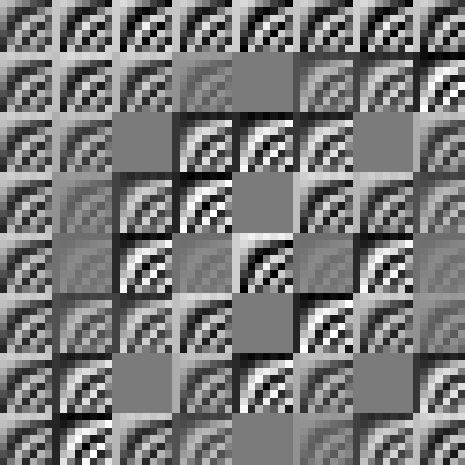
\includegraphics[width=.24 \linewidth]{figures/Basis.png}
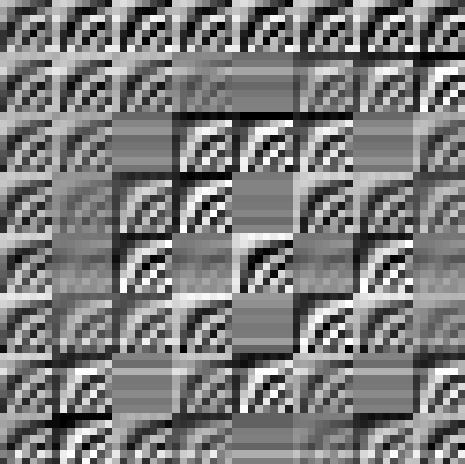
\includegraphics[width=.24 \linewidth]{figures/Ahat_FastICA_M640_K8_noise1_0205.png}
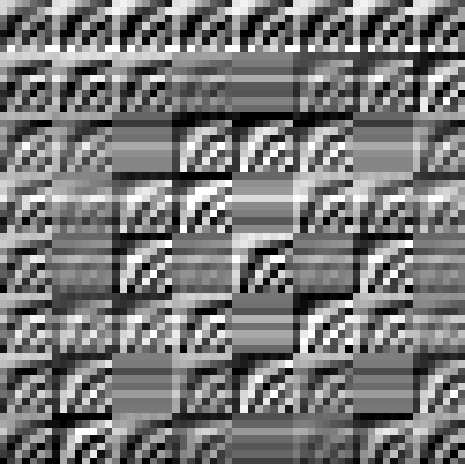
\includegraphics[width=.24 \linewidth]{figures/Ahat_FastICA_M640_K8_noise2_0409.png}
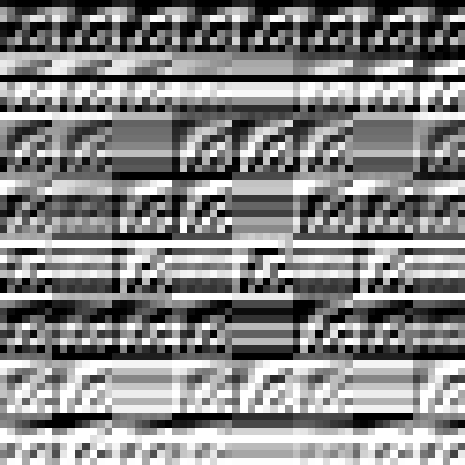
\includegraphics[width=.24 \linewidth]{figures/Ahat_FastICA_M640_K8_noise5_1021.png}
\caption{\textbf{Learning a dictionary from increasingly noisy data}. The (unraveled) basis elements of the $8 \times 8$ discrete cosine transform (DCT) form the 64 columns of the left-most matrix above. Three increasingly imprecise dictionaries (columns reordered to best match original) are recovered by FastICA \cite{hyvarinen2000independent} trained on data generated from $8$-sparse linear combinations of DCT elements corrupted with additive noise (increasing from left to right).}
\vspace{-.6 cm}
\label{noisyrecovery}
\end{center}
\end{figure}

\subsection{Probabilistic guarantees}

Another extension of Thm.~\ref{DeterministicUniquenessTheorem} can be derived from the following algebraic characterization of the spark condition.  Letting $\mathbf{A}$ be the $n \times m$ matrix of $nm$ indeterminates $A_{ij}$, the reader may work out why substituting real numbers for the $A_{ij}$ yields a matrix satisfying \eqref{SparkCondition} if and only if the following polynomial evaluates to a nonzero number:
\begin{align*}
f(\mathbf{A}) := \prod_{S \in {[m] \choose 2k}} \sum_{S' \in {[n] \choose 2k}} (\det \mathbf{A}_{S',S})^2,
\end{align*}
%
where for any $S' \in {[n] \choose 2k}$ and $S \in {[m] \choose 2k}$, the symbol $\mathbf{A}_{S',S}$ denotes the submatrix of entries $A_{ij}$ with $(i,j) \in S' \times S$.\footnote{The large number of terms in this product is likely necessary given that deciding whether or not a matrix satisfies the spark condition is NP-hard \cite{tillmann2014computational}.}

Since $f$ is analytic, having a single substitution of a real matrix $\mathbf{A}$ satisfying $f(\mathbf{A}) \neq 0$ implies that the zeroes of $f$ form a set of (Borel) measure zero. Such a matrix is easily constructed by adding rows of zeroes to a $\min(2k,m) \times m$ Vandermonde matrix as mentioned previously, so that every sum in the product defining $f$ above is strictly positive. Thus, almost every $n \times m$ matrix with $n \geq \min(2k,m)$ satisfies \eqref{SparkCondition}.

%Another extension of Thm.~\ref{DeterministicUniquenessTheorem} arises from the following analytic characterization of the spark condition.  Let $\mathbf{A}$  be the $n \times m$ matrix of $nm$ indeterminates $A_{ij}$. When real numbers are substituted for $A_{ij}$, the resulting matrix satisfies \eqref{SparkCondition} if and only if the following polynomial is nonzero:
%\begin{align*}
%f(\mathbf{A}) := \prod_{S \in {[m] \choose k}} \sum_{S' \in {[n] \choose k}} (\det \mathbf{A}_{S',S})^2,
%\end{align*}
%
%where for any $S' \in {[n] \choose k}$ and $S \in {[m] \choose k}$, the symbol $\mathbf{A}_{S',S}$ denotes the submatrix of entries $A_{ij}$ with $(i,j) \in S' \times S$.   We note that the large number of terms in this product is likely necessary due to the NP-hardness of deciding whether a given matrix $\mathbf{A}$ satisfies the spark condition \cite{tillmann2014computational}.

%Since $f$ is analytic, having a single substitution of a real matrix $\mathbf{A}$ with $f(\mathbf{A}) \neq 0$ necessarily implies that the zeroes of $f$ form a set of measure zero. Fortunately, such a matrix $\mathbf{A}$ is easily constructed by adding rows of zeroes to any $\min(2k,m) \times m$ Vandermonde matrix as described above (so that each term in the product above for $f$ is nonzero). Hence, almost every $n \times m$ matrix with $n \geq \min(2k,m)$ satisfies \eqref{SparkCondition}.

It turns out that a similar phenomenon applies to datasets of vectors with a stable sparse representation. Briefly, following the same procedure as in \cite[Sec.~IV]{Hillar15}, for $k < m$ and $n \geq \min(2k, m)$, we may consider the ``symbolic'' dataset $Y = \{\mathbf{A}\mathbf{x}_1,\ldots,\mathbf{A} \mathbf{x}_N\}$ generated by an indeterminate $n \times m$ matrix $\mathbf{A}$ and $m$-dimensional $k$-sparse vectors $\mathbf{x}_1, \ldots, \mathbf{x}_N$ indeterminate within their supports, which form a regular hypergraph $\mathcal{H} \subseteq {[m] \choose k}$ satisfying the SIP. Restricting \mbox{$(k-1){m \choose k} + 1$} indeterminate $\mathbf{x}_i$ to each support in $\mathcal{H}$, and letting $\textbf{M}$ be the $n \times N$ matrix with columns $\mathbf{A}\mathbf{x}_i$, it can be checked that when $f(\mathbf{M}) \neq 0$ for a substitution of real numbers for the indeterminates, all of the assumptions on $\mathbf{A}$ and the $\mathbf{x}_i$ in Thm.~\ref{DeterministicUniquenessTheorem} are satisfied. We therefore have the following.  % ; in particular, $\mathbf{A}$ satisfies \eqref{SparkCondition}

\begin{theorem}\label{robustPolythm}
%Let $\mathbf{A}$ and $\mathbf{x}_1, \ldots, \mathbf{x}_N$ be an indeterminate $n \times m$ matrix and sequence of $m$-dimensional vectors, respectively. 
There is a polynomial in the entries of $\mathbf{A}$ and the $\mathbf{x}_i$ that evaluates to a nonzero number only when $Y$ has a stable $k$-sparse representation in $\mathbb{R}^m$. In particular, almost all substitutions impart to $Y$ this property.
\end{theorem}

%To extend this observation to arbitrary probability distributions, note that if a set of measure spaces $\{(X_{\ell}, \nu_{\ell})\}_{\ell=1}^p$ has measures $\nu_{\ell}$ absolutely continuous with respect to the standard Borel measure on $\mathbb{R}$ for all $\ell \in [p]$, then the product measure $\prod_{\ell=1}^p \nu_{\ell}$ is also absolutely continuous with respect to the standard Borel product measure on $\mathbb{R}^p$ (e.g., see \cite{folland2013real}).  This fact combined with Thm.~\ref{robustPolythm} implies the following.
To extend this observation to arbitrary probability distributions, note that if a set of $p$ measure spaces has all measures absolutely continuous with respect to the standard Borel measure on $\mathbb{R}$, then the product measure is also absolutely continuous with respect to the standard Borel product measure on $\mathbb{R}^p$ (e.g., see \cite{folland2013real}).  This fact combined with Thm.~\ref{robustPolythm} implies the following.\footnote{We refer the reader to \cite{Hillar15} for a more detailed explanation of these arguments.}

\begin{corollary}\label{ProbabilisticCor}
If the indeterminate entries of $\mathbf{A}$ and the $\mathbf{x}_i$ are drawn independently from probability distributions absolutely continuous with respect to the standard Borel measure, then $Y$ has a stable $k$-sparse representation in $\mathbb{R}^m$ with probability one.
\end{corollary}

Thus, drawing the dictionary and supported sparse coefficients from any continuous probability distribution almost always generates data with a stable sparse representation.

%\cite{rehnsommer2007, rozell2007neurally, ganguli2012compressed, hu2014hebbian}

\section{Discussion}

It is befitting to comment on the optimality of these results. The linear scaling for $\varepsilon$ in \eqref{epsdel} is essentially optimal (e.g., see \cite{arias2013fundamental}), but a basic open problem remains: how many samples are necessary to determine the sparse coding model? 
These results demonstrate that sparse codes $\mathbf{x}_i$ drawn from only a polynomial number of $k$-dimensional subspaces permit stable identification of the generating dictionary $\mathbf{A}$. 
This lends some legitimacy to the use of the model in practice, where data in general are unlikely (if ever) to exhibit the exponentially many possible $k$-wise combinations of dictionary elements required by (to my knowledge) all previously published results. 

Consequently, if $k$ is held fixed or if the size of the support set of reconstructing codes is polynomial in $\overline m$ and $k$, then a practical (polynomial) amount of data suffices to identify the dictionary.\footnote{In the latter case, a reexamination of the pigeonholing argument in the proof of Thm.~\ref{DeterministicUniquenessTheorem} requires a polynomial number of samples distributed over a polynomial number of supports.} Reasons to be skeptical that this holds in general, however, can be found in \cite{tillmann2014computational, tillmann2015computational}. Even so, the next chapter contains a discussion on how probabilistic guarantees can in fact be made for any number of available samples.

As it seemed to benefit a reviewer of this work, some clarification may be in order on how the deterministic sample complexity $N = |\mathcal{H}|\left[(k-1){m \choose k} + 1\right]$ given here (Cor.~\ref{DeterministicUniquenessCorollary}) compares to those listed in the the top two rows listed in Table I of \cite{Hillar15}. To be clear, the theory developed here is strictly more general, since $\mathcal{H}$ can always be taken to be ${[m] \choose k}$. The point of difference in this comparison is the assumed set of supports for sparse codes, which is always ${[m] \choose k}$ in \cite{Hillar15}, whereas here it can be assumed to be any regular $k$-uniform hypergraph that satisfies the SIP. By row, %, assuming for our results that sufficient data have been sampled from all supports in a hypergraph H satisfying the SIP:
\begin{enumerate}
\item[I.] The result here improves upon the listed $k{m \choose k}^2$ by an exponential factor, since for every $k < m$ there exists a regular $k$-uniform hypergraph $\mathcal{H}$ with $|\mathcal{H}| = m$ satisfying the SIP. 
\item[II.] The authors in \cite{Hillar15} have applied measure-theoretic arguments to achieve $(k+1){m \choose k}$ with almost-certainty (i.e. with probability one), a factor of $m$ reduction over that for which certainty can alternatively be guaranteed here.    
%\item[III.] A direct comparison cannot be made because it is an open question as to the probability that a random set of supports satisfies the SIP. This would be an interesting problem for the community to solve; regardless, the result of \cite{Hillar15} is still implied by the more general theory given here.
%\item[IV.] The result here is $|\mathcal{H}\left[|(k-1){m \choose k} + 1\right]$ with probability one compared to $(k+1){m \choose k}$ with probability one. In this case the sample complexity stated in \cite{Hillar15} is marginally better, but it relies on a noise-free technicality unique to their assumption $\mathcal{H} = {m \choose k}$. %differs in flavor: their $\mathbf{x_i}$ are assumed to be distributed as $(k+1)$ samples per support for every support of size $k \in [m]$, whereas here it is assumed that $(k-1){m \choose k}$ codes $\mathbf{x_i}$ are distributed over each support in some hypergraph $\mathcal{H}$ satisfying the SIP. 
%\item[V.] Again, a direct comparison cannot be made for the reason stated for row III.
\end{enumerate}
